%=====================================================================
\section{Evidence so far}
\label{sec:evidence}

\subsection{Verification of the implementation}

\code{test\_rl2.py} (identical to RL1's tests plus check 6) is run before every training:
\begin{enumerate}
  \item \textbf{Data.} The CSV loader builds exactly the instance of the MILP's text loader (RL1 full test: all 228 tested instances, 56 files $\times$ $n=10/50/100$ plus 60 Gehring--Homberger files at $n=200$).
  \item \textbf{Simulator.} The greedy cost rule played inside the simulator gives the same plan cost as \code{greedy\_f3} of the MILP code, and the simulator's $Z$ equals the checker's $Z$ (RL1: 190 instances).
  \item \textbf{Random policy.} Plans of an untrained network without dropped EVs pass the checker with no violation and the same $Z$ as the simulator; plans with dropped EVs are complete and flagged.
  \item \textbf{Generator.} Random instances of every class run through simulator and checker.
  \item \textbf{Training step.} Finite loss and gradients.
  \item \textbf{Active search (RL2).} Replaying the incumbent's actions rebuilds the same plan; a few iterations never return a worse plan; the starting embeddings are left untouched; the plan passes the checker.
\end{enumerate}
All six checks passed on the laptop (22 Nov 2026, quick mode); a 2-epoch training run and the comparison script ran end to end.

\subsection{RL1 training on the server}

RL1 was trained on an RTX 4090 (torch 2.14.1, CUDA 12.6) on 22 Nov 2026. Figure~\ref{fig:train} shows the validation ratio by $n$.

\begin{figure}[h]
\centering
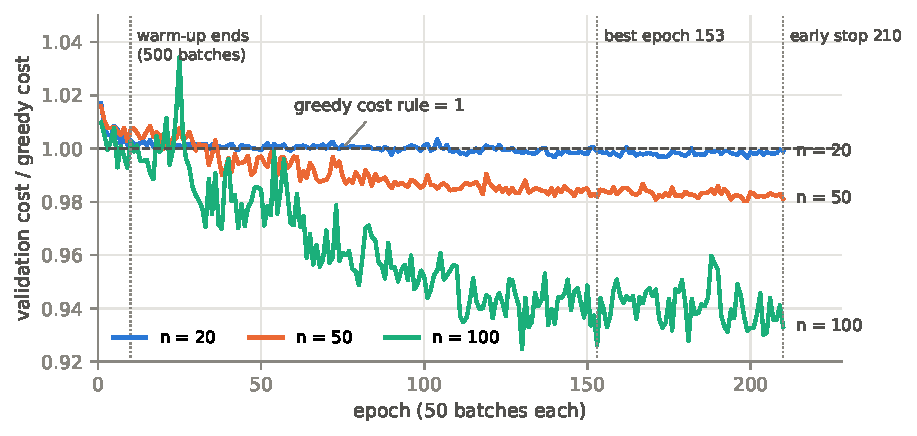
\includegraphics[width=0.9\textwidth]{figures/rl1_training_curve.pdf}
\caption{RL1 validation ratio (policy cost / greedy-rule cost, below 1 = better than the rule) per epoch, for $n=20$, $50$, $100$. Epoch 0 (untrained, 1.43 overall) is off the scale.}
\label{fig:train}
\end{figure}

\begin{itemize}
  \item Untrained: ratio 1.43. After the first warm-up epoch (50 imitation batches): 1.014.
  \item REINFORCE from epoch 11 lowered the ratio steadily to about 0.98 by epoch 75 and 0.969 at epoch 153 (best). The gain is almost entirely at large $n$: at $n=100$ the ratio fell to about 0.93, at $n=20$ it stayed near 1.00 (small instances leave little room beyond the rule).
  \item After epoch 150 the ratio moved between 0.970 and 0.975 without a new best; training stopped early at epoch 210 (10 epochs without improvement after the first 200). Total 10\,500 batches in 38.6 minutes.
\end{itemize}

\subsection{RL1 on the 560 test instances}

\begin{table}[h]
\centering\small
\caption{RL1 against the 300-second MILP and the greedy rule, by Solomon class. Gaps are $100(Z_{\text{RL1}}-Z_{\text{other}})/Z_{\text{other}}$ over instances where both plans are valid.}
\label{tab:rl1class}
\begin{tabular}{@{}lrrrrrrr@{}}
\toprule
class & inst. & \shortstack[r]{RL1\\valid} & \shortstack[r]{MILP\\valid} & \shortstack[r]{RL1 valid,\\MILP none} & \shortstack[r]{gap to\\MILP \%} & \shortstack[r]{gap to\\optimum \%} & \shortstack[r]{gap to\\greedy \%} \\
\midrule
C1 & 90 & 90 & 90 & 0 & 1.06 & 0.74 & $-1.12$ \\
C2 & 80 & 80 & 79 & 1 & 1.60 & 1.44 & $-1.04$ \\
R1 & 120 & 89 & 76 & 13 & 0.80 & 0.34 & $-1.96$ \\
R2 & 110 & 110 & 110 & 0 & 1.22 & 0.66 & $-2.57$ \\
RC1 & 80 & 53 & 44 & 9 & 1.13 & 0.75 & $-5.94$ \\
RC2 & 80 & 80 & 80 & 0 & 0.60 & 0.19 & $-4.01$ \\
\midrule
all & 560 & 502 & 479 & 23 & 1.07 & 0.74 & $-2.47$ \\
\bottomrule
\end{tabular}
\end{table}

\begin{itemize}
  \item \textbf{Feasibility.} RL1 finds a valid plan in 502 instances, the MILP in 479. In 23 instances (R1, RC1, one C2) RL1 has a valid plan where the MILP found none in 300 s; the reverse never happens. Of the 58 instances without an RL1 plan, 51 are proven infeasible (the data), so RL1 misses at most 7.
  \item \textbf{Cost.} Where both have a valid plan, RL1 is 1.07\,\% dearer than the MILP on average (median 0.89\,\%), 0.74\,\% above proven optima, and 2.47\,\% cheaper than the greedy rule (better in 366 of 474 instances).
  \item \textbf{Time.} 0.12 s per instance (520 rollouts) against 150.7 s for the MILP: about 1\,250 times faster.
  \item \textbf{Where it loses.} The gap grows with $n$ up to $n=80$ (Figure~\ref{fig:gapn}) and is largest in class C2 (long period, clustered customers).
\end{itemize}

\begin{figure}[h]
\centering
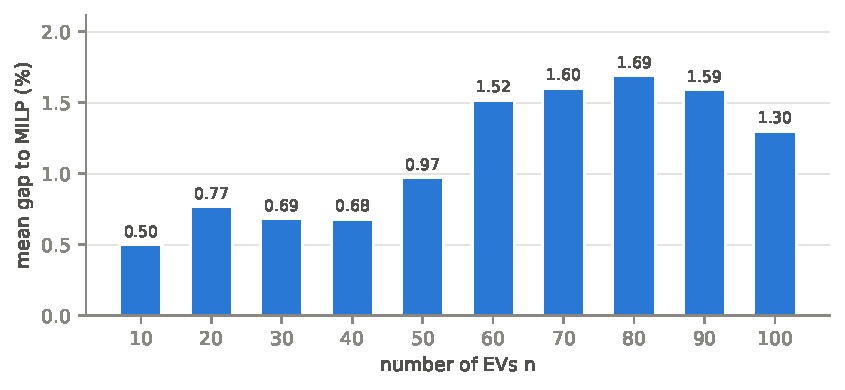
\includegraphics[width=0.85\textwidth]{figures/rl1_gap_by_n.pdf}
\caption{RL1 mean gap to the MILP plan by number of EVs (instances where both plans are valid). This profile motivated RL2's size weighting and active search.}
\label{fig:gapn}
\end{figure}

\subsection{Evidence behind RL2}

\textbf{More sampling helps little.} On seven test instances, sampling 8 times more plans per symmetry (512 instead of 64, i.e.\ 4\,104 plans instead of 520) lowered RL1's mean gap to the MILP only from 1.83\,\% to 1.43\,\%: the trained policy keeps proposing plans from the same region.

\textbf{Active search helps a lot.} Active search on RL1's trained model (the ablation of Section~\ref{sec:eas}; laptop CPU, only 30 iterations, RL1's files only read) on the three instances with the largest gaps:

\begin{center}\small
\begin{tabular}{@{}lrrrr@{}}
\toprule
instance & sampling (520 plans) & $8\times$ more sampling & active search & change in $Z$ \\
\midrule
EV-R208, $n=60$ & 3.92\,\% & 3.25\,\% & 1.25\,\% & $-2.57$\,\% \\
EV-C104, $n=90$ & 2.59\,\% & 0.97\,\% & 0.81\,\% & $-1.74$\,\% \\
EV-R112, $n=80$ & 1.76\,\% & -- & $-0.23$\,\% & $-1.96$\,\% \\
\midrule
mean gap to MILP & 2.76\,\% & & 0.61\,\% & \\
\bottomrule
\end{tabular}
\end{center}
On EV-R112 the searched plan is cheaper than the MILP's 300-second plan. The best plans were found late (iterations 23--28 of 30), so more iterations should help further; on the CPU an iteration took 6--14 s, while on the GPU it is expected to take a fraction of a second (not yet measured), so the 10-second cap should allow far more than 30.

These numbers are from three instances and must not be read as the expected average; they are the reason RL2 was built, not its result.

\subsection{What the RL2 server run will show}

\code{compare\_rl2.py} reports, per method (RL2-EAS, RL2, RL1, greedy) against the MILP: valid plans, plans where the MILP has none, mean and median gap to the MILP and to proven optima, wins against greedy, and seconds per instance, overall, by class and by $n$, plus what active search changed. Two comparisons answer the two questions of RL2:
\begin{itemize}
  \item \code{rl2\_sampling} vs \code{rl1}: did the new training (batch 64, $P(n)\propto n$, larger validation) help, especially at $n\ge60$?
  \item \code{rl2\_eas} vs \code{rl2\_sampling}: how much does active search add, and at what time cost (at most 10 s per instance)?
\end{itemize}
